\documentclass[a4paper,11pt]{article}

\usepackage[latin1]{inputenc}
\usepackage[T1]{fontenc}
\usepackage{bbm} %math chars
\usepackage{amsmath}
\usepackage{indentfirst}
\usepackage{fullpage} %minimizes the default margins
\usepackage{url}
\usepackage{graphicx}
\usepackage[center,footnotesize]{caption} %options des legendes des graphes
\usepackage[section]{placeins} %place les figures d'une section avant le debut de la suivante
\usepackage{subfig} %a) b) c)

\title{Series 5}
\date{}
\author{Genomics and bioinformatics - Week 6 - October 23, 2012}

\begin{document}
\maketitle

\section{Phylogenetic trees}

\begin{enumerate}
\item 
\begin{center}
\includegraphics[width=0.8\textwidth]{tree.png}\\
\vspace{0.5cm}
{\bf The gene tree}
\end{center}

\item
\begin{itemize} 
\item An orthologous pair: {\bf dr\_per2} and {\bf mm\_per2}

\item A paralogous pair in the same species: {\bf mm\_per1} and {\bf mm\_per2}

\item A paralogous pair in different species: {\bf mm\_per1} and {\bf dr\_per2}
\end{itemize}
\end{enumerate}

\section{Another HMM}

\subsection{The Viterbi algorithm}

\begin{center}
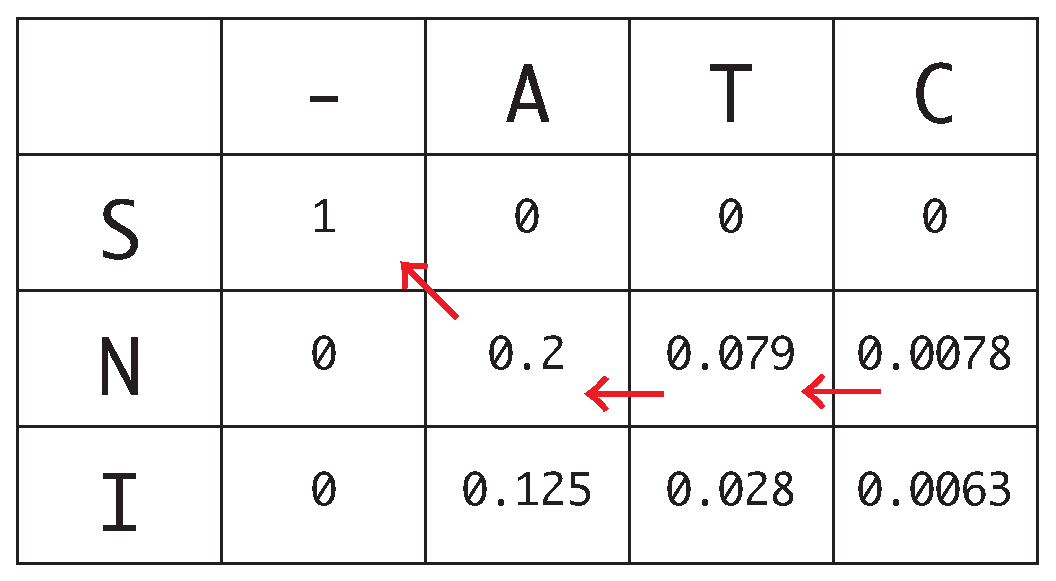
\includegraphics[width=0.7\textwidth]{fig3.eps}\\
\vspace{0.5cm}
{\bf The Table}
\end{center}

%\subsection{Using R}

%Comments...

\end{document}











